\section{Transformer - Run-time Reconfigurable Heterogeneous Architecture}
\label{sec_arch}


\subsection{Architecture Overview}

Figure \ref{fig_arch} shows the {\em Transformer}, a heterogeneous
architecture for transparent acceleration of dynamic
workloads. The {\em Transformer} consists of cores with private L1 caches along with a
partial reconfigurable logic unit, also referred to as a programmable
accelerator within the context of this paper, for instantiating acceleration
functions. The reconfigurable logic, equipped with input and output
buffers, shares the L2 cache with the cores through dedicated DMA
channels. All processing elements, including the cores and the accelerator, are
interconnected by way of a mesh-type network on the chip (NoC). The memory
hierarchy, consisting of the private memory units for both the cores and the accelerator,
 along with the shared L2 cache and the main memory, follows the MOESI protocol in order to maintain
coherence.

\begin{figure}
    \centering
    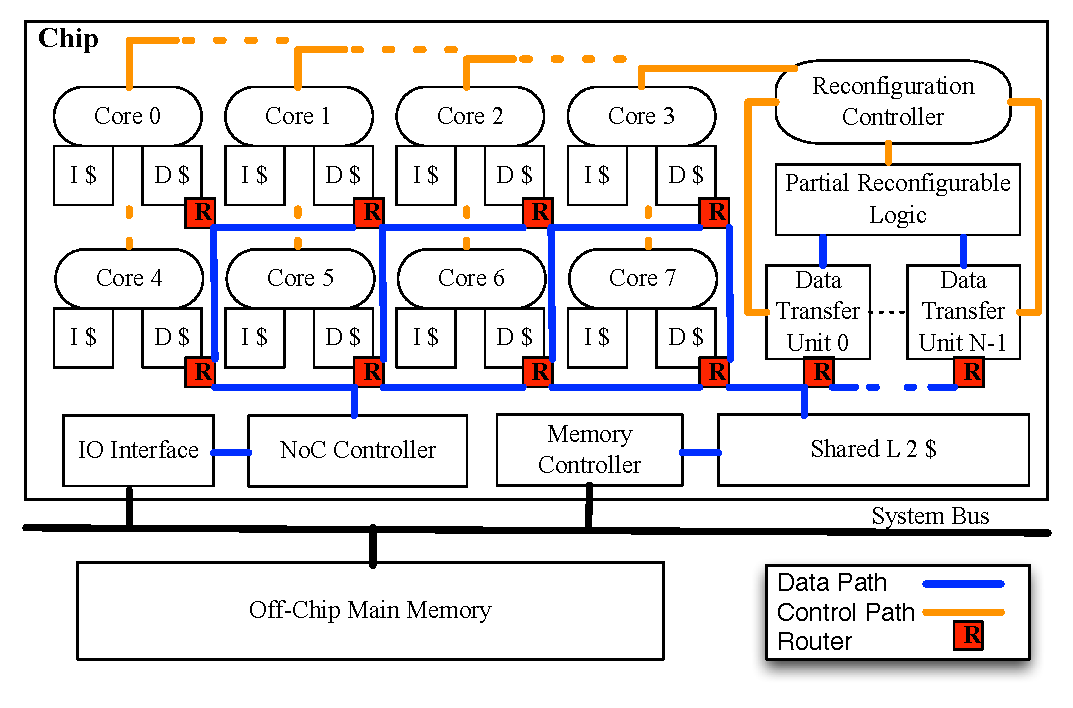
\includegraphics[width=4.0 in]{HPCA14-arch}
    \caption{Architecture Overview of {\em Transformer} }
    \label{fig_arch}
\vspace{-0.05in}
\end{figure}

The {\em Transformer}'s reconfigurable logic consists of the computational resources
and the {\em N} data transfer
units, which supports the instantiation of {\em N} independent accelerator
functions. The computational resources are organized in BRAM, DSP,
as well as SLICEs as in a generic FPGA chip. The actual number of functions instantiated within the
programmable logic depends on the particular functions selected to be
sped up at runtime and the resource requirements of the hardware
implementation for these functions. We study the architectural trade-offs of 
the reconfigurable logic and the number of cores in terms of performance
gains and power savings in Section \ref{sec_perf}.

Figure \ref{fig_reconfig_controller} depicts the three key components
in controlling the reconfiguration of the accelerator logic:
the reconfiguration controller, the reconfigurable logic and the data transfer
units. The reconfiguration controller is responsible for programming
new functions into the reconfigurable logic through new bit streams or
partial reconfiguration. By using the control and status registers to record the
status of the reconfiguration logic, the controller receives
instructions from the middleware running on one of the cores, tracks
demands for the various function calls, and makes decisions on what functions to accelerate and
when to accelerate them.

The reconfigurable logic consists of a static region, a Partial
Reconfigurable Region (PRR) and an Internal Configuration Access Port
(ICAP). The static region contains the necessary logic outside of the
accelerator PRMs, including the clock module, the interconnection interface and the
memory control interface. The PRR can be divided into smaller
sub-regions and configured on demand with different partial bit streams. ICAP is notified by the reconfiguration controller regarding
the type of accelerator 
%PRMs ({\bf FIXME all different PRMs are located in
%  their fixed addresses}) 
that should be configured and when it should start. In response, ICAP notifies
the controller with a "resource full" or a "(re)configuration done" message by
writing to the specific bits of the control registers.

Each data transfer unit includes a pair of input and output buffers
that can be filled or drained by a DMA engine. The DMA engine is
responsible for the bulk data transfers between the L2 cache and the
IO buffers, which are used as a form of scratchpad memory in order for the
reconfigurable logic to complete the necessary operations on the data. Other
parameters such as the memory addresses and the data size of the DMA
operations are passed by the reconfiguration controller. The TLBs on each
of the data transfer units are responsible for translating virtual
memory addresses into physical memory addresses.


\begin{figure}
    \centering
    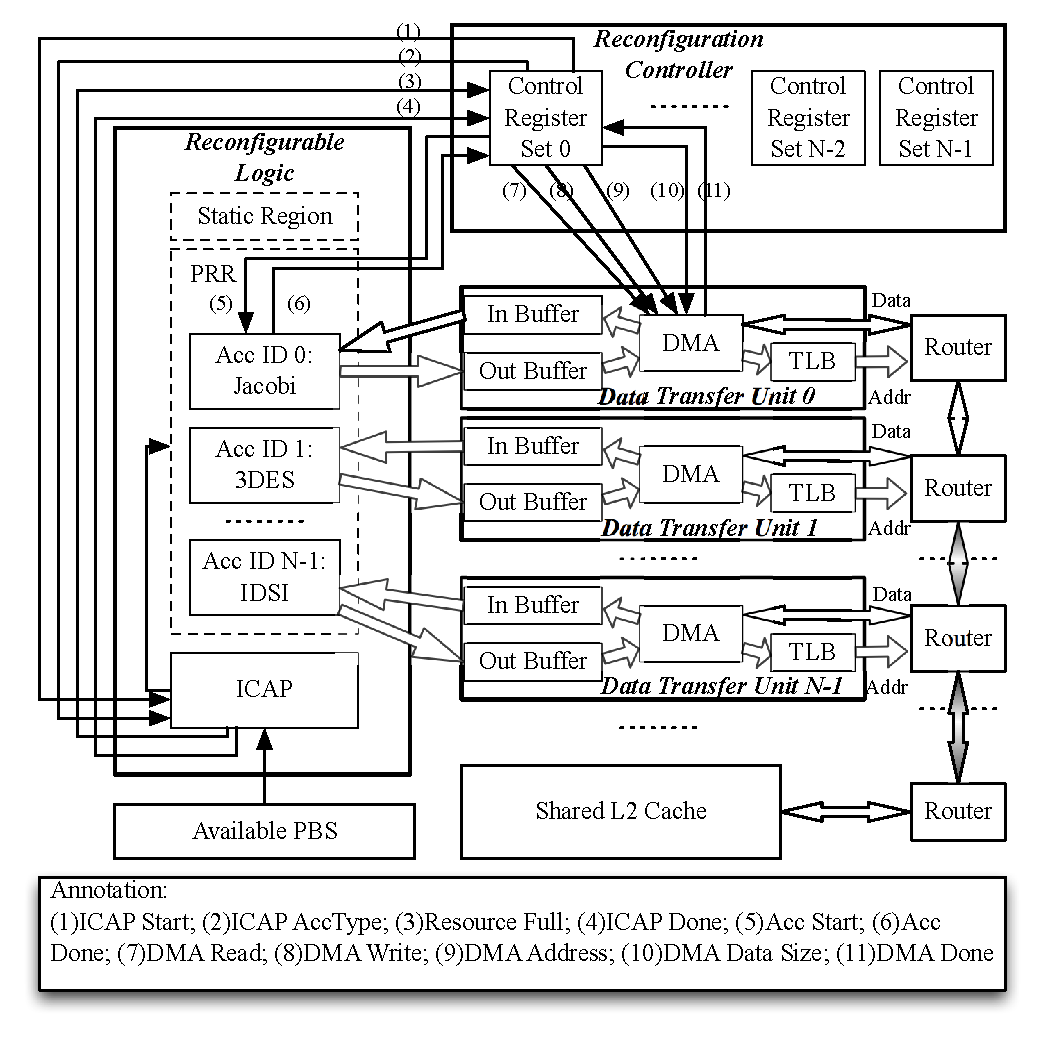
\includegraphics[width=4.0 in]{HPCA14-Controller}
    \caption{Transformer's Reconfigurable Logics and Controller}
    \label{fig_reconfig_controller}
\vspace{-0.05in}
\end{figure}


\subsection{Accelerator Invocation}

The invocation of the accelerator from the software executing within a given core is
done with specific accelerator instructions along with the control as well as the status
registers. We illustrate how the accelerator is invoked in Figure
\ref{fig_Acc_Invoc}. We introduce {\em N} control register sets for
each accelerator to be instantiated along with two new instructions to
invoke the core-to-accelerator as well as the accelerator-to-core execution path
transitions. Each control register set contains three 32-bit registers, including the
general control register, the DMA read register and the DMA write
register. The general control register is responsible for ICAP control,
acceleration control, and DMA control. The DMA read and write registers
contain the read and write addresses for the corresponding DMA operation source and destination
addresses. The specifications of the registers are described in Table
\ref{tbl_AccReg} while the two new instructions are listed below.

\begin{enumerate}
\item{\em readreg n}: read control register set with ID n.
\item{\em writereg n}: write the value into control register set with ID n.
%\item{\em accload AccReg n}: start configuring the type of accelerator
%  bitstream indicated by AccReg n into the reconfigurable logic. 
\end{enumerate}

\begin{table}[ht]
\scriptsize
\begin{center}
\begin{tabular}{|l|l|l|}
\hline 
\textbf{Register Name} & \textbf{Bits} & \textbf{Function}\\ 
\hline 
\hline
General Control &{\em Bit 0}   & ICAP start bit (IS)\\ 
\hline 
 &{\em Bit 1}   &  ICAP done bit (ID)\\ 
\hline 
 &{\em Bit 2-6} & ICAP accelerator type (IT 0-4)\\ 
\hline 
 &{\em Bit 7}   & acceleration start bit (AS)\\ 
\hline 
 &{\em Bit 8}   & acceleration done bit (AD)\\ 
\hline 
 &{\em Bit 9}   & DMA read enable (RE)\\ 
\hline 
 &{\em Bit 10}  & DMA write enable (WE)\\ 
\hline 
 &{\em Bit 11}  & DMA done (DD)\\
\hline
 &{\em Bit 12-15} & accelerator ID (ID 0-3)\\
\hline
 &{\em Bit 16-31} & DMA data block size (DS 0-15)\\
\hline
DMA Read Control &{\em Bit 0-31}  & DMA read address (RA 0-31)\\
\hline
DMA Write Control &{\em Bit 0-31} & DMA write address (WA 0-3)\\
\hline
\end{tabular} 
\caption{Control Registers for Reprogramming Accelerators.}
\label{tbl_AccReg}
\end{center}
\end{table}

The following is a brief introduction to intricacies of invoking the accelerator. 
Note that all the set and reset operations are done by using the
{\em readreg} and the {\em writereg} instructions. The aforementioned instructions are
encapsulated within customized wrapper functions, instead of being
used directly within a given user application.

\begin{enumerate}
\item If the reconfigurable controller decides to configure a specific
  combination of functions, based upon knowledge derived from the middleware, the
  middleware will set the ICAP Start (IS) bit in order to initiate the
  reconfiguration process using the corresponding functions identified by ICAP
  accelerator type (IT 0-4). (Note that the loading process will be skipped if
  the function is already configured within the accelerator logic.) At the
  same time, the middleware will prepare the data address and the data
  block size by writing the DMA read address (RA 0-31) bits and DMA
  data block size (DS 0-15) bits.

\item In addition to the reconfiguration process, we set the DMA Start
  (DS) bit in order to initiate reading data from the shared L2 cache or main
  memory into the accelerator local input buffer until the buffer is full.

\item When the reconfiguration is done, ICAP will set the ICAP Done
  (ID) bit to enable the start of the acceleration. By setting
  the acceleration start (AS) bit, the Reconfiguration Controller causes a
  thread context switch on the corresponding core, which begins the
  execution of a different thread. The suspended thread will sleep
  until the acceleration done (AD) bit is set.

\item When the acceleration function has completed or the middleware
  decides to erase and change the accelerator function for the core,
  the AccDone (AD) bit will be set and an interrupt will be generated in order to
  wake up the sleeping thread. Afterwards, the core will resume the previously
  inactive thread, which will either continue a software path or get
  ready for the next accelerator invocation.
\end{enumerate}


\begin{figure}
    \centering
    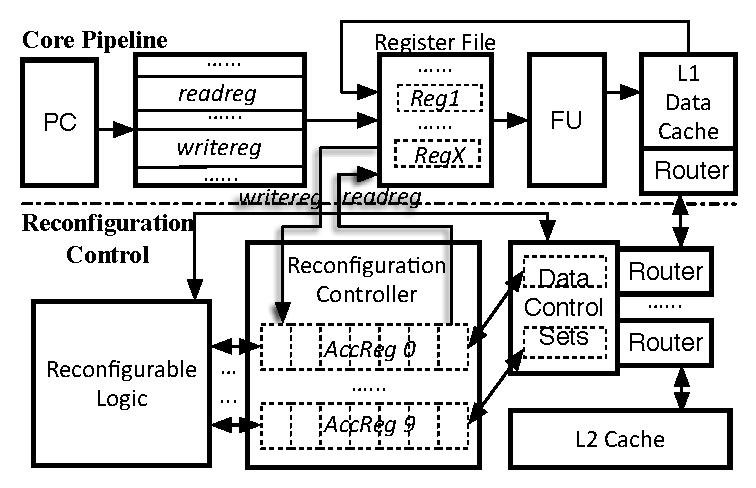
\includegraphics[width=4.0 in]{HPCA14-Acceleration_Invocation}
    \caption{Acceleration Invocation.}
    \label{fig_Acc_Invoc}
\end{figure}


In order to reduce the data transaction time between the accelerators, a
combination of DMA and double buffering is used. 
By using double buffering, the accelerators can work on data residing in
their local memory while the DMA is fetching the next batch of data. A
TLB is located in between the DMA cache as well as the L2 cache in order to perform
virtual-to-physical address translation. The aforementioned mechanism simplifies the
accelerator design and guarantees process isolation.
